\section{Integrali impropri}
\subsection{Integrazione secondo Riemann}

Data $f:[a,b] \rightarrow \mathbb{R}$ limitata, con $a=x_0 < x_1 < \ldots < x_n =b$ e $[a,b]$ intevallo limitato:
\begin{gather*}
	S(f) =\sum_{i=1}^{n} \left( \sup_{[x_{i-1},x_i]} f(x) \right) \cdot (x_i-x_{i-1}) \qquad \text{somma superiore}
	\\
	s(f) =\sum_{i=1}^{n} \left(\inf_{[x_{i-1},x_i]} f(x)\right)\cdot (x_i-x_{i-1}) \qquad \text{somma inferiore}
\end{gather*}
Se $\inf_{a=x_0 < x_1 < ... < x_n =b} S(f) = \sup_{a=x_0 < x_1 < ... < x_n =b} s(f) =I \in \mathbb{R}$ allora $f$ si dice Riemann integrabile in $[a,b]$ e si pone 
\begin{equation*}
	\int_{a}^{b} f(x) \mathrm{d}x=I.
\end{equation*}


\subsubsection{Integrali impropri}
\begin{exbar}
\begin{example}
	\begin{equation*}
		f(x)=\frac{1}{x^\alpha}, \qquad x \geq 1, \; \alpha \in \mathbb{R}
	\end{equation*}
	
	Vogliamo definire, se possibile, 
	\begin{equation*}
		\int_{1}^{+\infty} f(x) \ \mathrm{d}x= \int_{1}^{+\infty}\frac{1}{x^\alpha} \ \mathrm{d}x
	\end{equation*}
	Stiamo provando ad integrare una funzione limitata su un intervallo illimitato.
	
\begin{comment}
	\begin{figure}[h!]
		\centering
		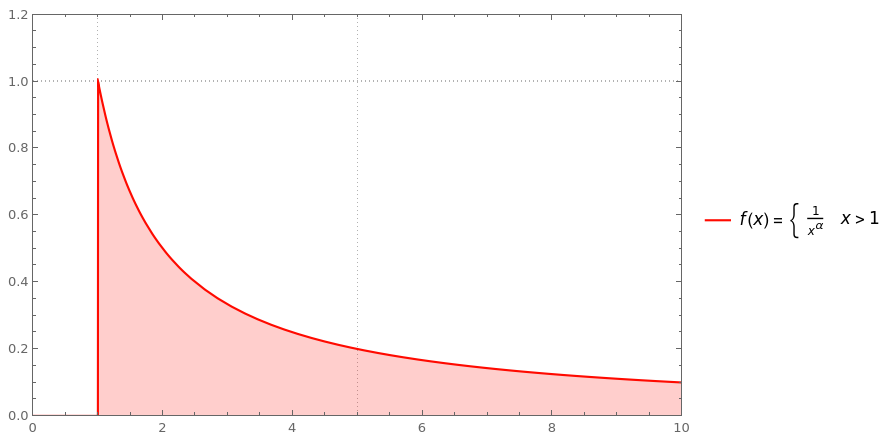
\includegraphics[width=\textwidth]{unosuxallaalpha.png}
	\end{figure}
	
	Fissato $c > 1$, riesco a definire $\int_{1}^{c} f(x)dx$ perchè integro una funzione limitata su un intervallo limitato.\\
	Posso dunque definire
	\begin{empheq}{align*}
		\int_{1}^{+\infty} f(x)dx &=\lim_{c\rightarrow +\infty} \int_{1}^{c}f(x)dx, \,\,\,\,\, \text{se}\,\,\, \exists\\
		\int_{1}^{+\infty} \frac{1}{x^\alpha} dx &= \lim_{c \rightarrow + \infty}\int_{1}^{c} \frac{1}{x^\alpha}dx\\
		&=
		\begin{cases}
			& \lim_{c \rightarrow +\infty}\frac{1}{1-\alpha}[c^{1-\alpha}-1]\,\,\,\, \text{se}\,\,\, \alpha \neq 1\\
			& \lim_{c \rightarrow +\infty} \ln c \,\,\,\, \text{se} \,\,\, \alpha=1
		\end{cases}\\
		&=
		\begin{cases}
			& \frac{1}{\alpha-1} \,\,\,\, \text{se} \,\,\, \alpha > 1\\
			&+\infty \,\,\,\, \text{se} \,\,\, \alpha \leq 1
		\end{cases}
	\end{empheq}
	
	\paragraph{\textcolor{red}{Esempio}}
	\begin{empheq}{equation*}
		f(x)=-\ln x, \,\,\, x \in ]0,1]
	\end{empheq}
	e provo a definire 
	\begin{empheq}{equation*}
		\int_{0}^{1} f(x)dx
	\end{empheq}
	cioè l'integrale di una funzione illimitata su un intervallo limitato.\\
\end{example}
\end{exbar}


	
	

	


	

	

	
	\begin{figure}[h!]
		\centering
		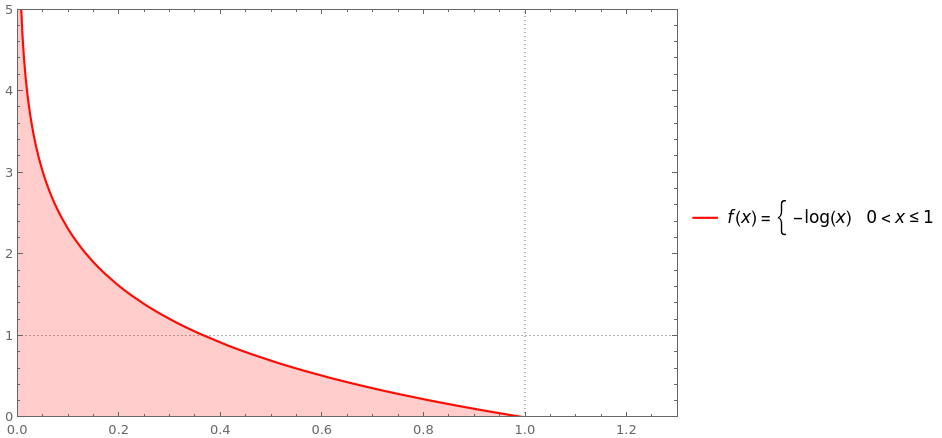
\includegraphics[width=\textwidth]{intda1a0.png}
	\end{figure}
	Riesco a definire bene $\int_{c}^{1} f(x)dx$ perchè integro una funzione limitata
	\textcolor{orange}{$(|f(x)|\leq -\ln c \forall x\in[c,1])$} su un intervallo limitato.\\
	Posso dunque definire
	\begin{empheq}{align*}
		\int_{0}^{1} f(x)dx &= \lim_{c\rightarrow +0^+} \int_{c}^{1} f(x)dx\,\,\,\,\,\, \text{se}\,\,\, \exists\\
		\int_{0}^{1}(-\ln x) dx &= \lim_{c \rightarrow 0^+} \int_{c}^{1}(-\ln x)dx\\
		&= \lim_{c \rightarrow 0^+} [x-x\ln x]_{c}^{1} \\
		&= \lim_{c \rightarrow 0^+} [1-c+c\ln c]=1
	\end{empheq}
	
	\paragraph{\textcolor{red}{Definizione}}
	Sia $f:[a,b[\rightarrow \R, a,b \in \R \cup\{+\infty\}$ \textcolor{orange}{(voglio definire $\int_{a}^{b}f(x)dx$)} Riemann integrabile in $[a,c]\,\, \forall c \in [a,b[$. Se $\exists$ finito il $\lim_{c \rightarrow b^-} \int_{a}^{c}f(x)dx $, allora $f$ si dice integrale in senso improprio o generalizzato in $[a,b[$ e la quantità 
	\begin{empheq}{equation*}
		\int_{a}^{b} f(x)dx = \lim_{c\rightarrow b^-} \int_{a}^{c} f(x)dx
	\end{empheq}
	si dice integrale improprio o generalizzato di $f$ in $[a,b[$.\\
	Analogamente, data $f:]a,b]\rightarrow \R, a,b \in \R \cup \{-\infty\}$, Riemann integrabile in $[c,b]\,\, \forall c \in ]a,b]$. Se $\exists$ finito il $\lim_{c \rightarrow a^+} \int_{c}^{b} f(x)dx$, allora $f$ si dice integrabile in senso improprio o generalizzato in $]a,b]$ e la quantità
	\begin{empheq}{equation*}
		\int_{a}^{b} f(x)dx = \lim_{c \rightarrow a^+} \int_{c}^{b} f(x)dx
	\end{empheq}
	si dice integrale improprio o generealizzato di $f$ in $]a,b]$.\\
	Se $f$ è integrabile in senso improprio in un intervallo $I$, allora si dice anche che l'integrale (improprio) di $f$ in $I$ è convergente o che $f$ ha integrale (improprio) convergente in $I$.\\
	Se il limite che definisce l'integrale improprio di $f$ è infinito, si dice anche che l'integrale (improprio) di $f$ è divergente o che $f$ ha integrale (improprio) divergente in $I$.
	
	\paragraph{\textcolor{red}{Osservazione}}
	Vista la definizione, 
	\begin{empheq}{equation*}
		\int_{1}^{+\infty}\frac{1}{x^\alpha}dx \,\,\,\,\, \text{converge} \Leftrightarrow \alpha > 1
	\end{empheq}
	
	\paragraph{\textcolor{red}{Esempio Importante}}
	\begin{empheq}{equation*}
		f(x)=\frac{1}{(x-a)^\alpha}, \,\,\,\, x \in ]a,a+1], \,\,\, a\in \R \,\, \text{fissato},\,\,\, \alpha\in\R\,\,\, \text{parametro},\,\,\, \alpha > 0
	\end{empheq}
	Studiamo la convergenza di 
	\begin{empheq}{align*}
		\int_{a}^{a+1} \frac{1}{(x-a)^\alpha} dx  &= \lim_{c \rightarrow a^+} \int_{c}^{a+1} \frac{1}{(x-a)^\alpha} dx\\
		&=
		\begin{cases}
			& \lim_{c \rightarrow a^+} \frac{1}{1-\alpha}[1-(c-a)^{1-\alpha}] \,\,\,\, \text{se}\,\, \alpha \neq 1 \\
			& \lim_{c \rightarrow a^+} -\ln(c-a)\,\,\,\, \text{se} \,\, \alpha =1
		\end{cases}\\
		&=
		\begin{cases}
			& \frac{1}{1-\alpha} \,\,\,\, \text{se}\,\, \alpha <1 \\
			&+\infty \,\,\,\, \text{se}\,\, \alpha \geq1.
		\end{cases}
	\end{empheq}
	Dunque 
	\begin{empheq}{equation*}
		\int_{a}^{a+1} \frac{1}{(x-a)^\alpha} dx \,\,\,\, \text{converge} \Leftrightarrow \alpha < 1.
	\end{empheq}
	In particolare
	\begin{empheq}{equation*}
		\int_{0}^{1} \frac{1}{x^\alpha} \,\,\,\, \text{converge} \Leftrightarrow \alpha < 1.
	\end{empheq}
	
	\paragraph{\textcolor{red}{Esempio}}
	Stabilire se converge 
	\begin{empheq}{equation*}
		\int_{0}^{1} \frac{\sin{\frac{1}{x}}}{x^2} dx
	\end{empheq}
	\begin{figure}[h!]
		\centering
		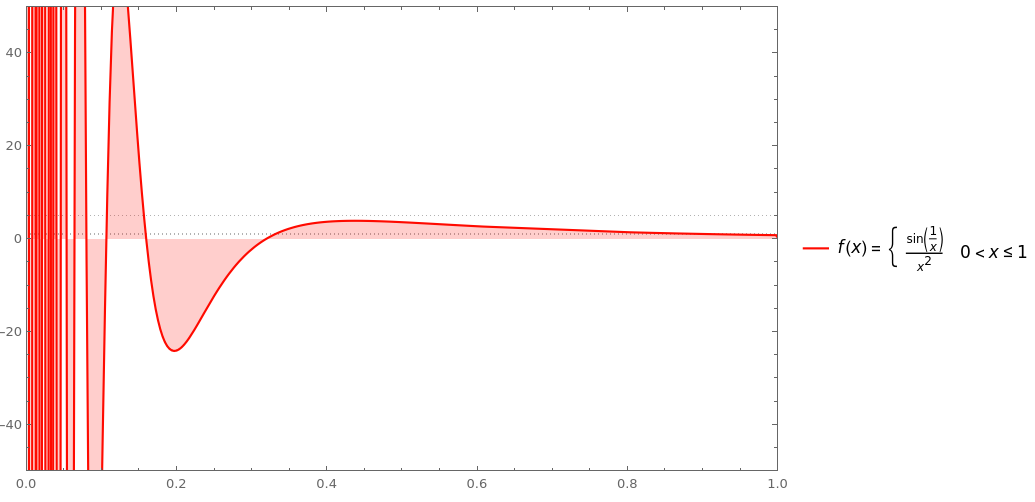
\includegraphics[width=\textwidth]{senobuffo.png}
	\end{figure}
	
	Devo calcolare 
	\begin{empheq}{equation*}
		\lim_{c\rightarrow0^+} \int_{c}^{1} \frac{\sin{\frac{1}{x}}}{x^2} dx= \lim_{c \rightarrow 0^+} \cos{\frac{1}{x}}|_{c}^{1}=\lim_{c\rightarrow 0^+}\left(1-\cos{\frac{1}{c}}\right)
	\end{empheq}
	che non esiste $\Rightarrow$ la funzione $f(x)=\frac{\sin{\frac{1}{x}}}{x^2}$, non è integrabile in senso improprio in $]0,1]$.
	
	\paragraph{\textcolor{red}{Esempio Importante}}
	\begin{empheq}{align*}
		\int_{0}^{+\infty} e^{\alpha x} dx &=\lim_{c \rightarrow +\infty} \int_{0}^{c} e^{\alpha x} dx \\&= \lim_{c \rightarrow +\infty} \frac{1}{\alpha}(e^{\alpha c}-1)\\
		&= \begin{cases}
			& -\frac{1}{\alpha} \,\,\,\, \text{se} \,\, \alpha <0\\
			&+\infty \,\,\,\, \text{se} \,\, \alpha >0.
		\end{cases}
	\end{empheq}
	\begin{empheq}{equation*}
		\int_{0}^{+\infty} e^{\alpha x} \,\,\,\,\, \text{converge} \Leftrightarrow \,\,\, \alpha <0.
	\end{empheq}
	Analogamente
	\begin{empheq}{equation*}
		\int_{-\infty}^{0} e^{\alpha x} dx \,\,\,\,\, \text{converge} \Leftrightarrow \,\,\, \alpha > 0.
	\end{empheq}
	Dato $ a>0$, scrivendo $e^{\alpha x} = e^{(\alpha \ln a)x}$ si deduce la convergenza degli integrali
	\begin{empheq}{align*}
		&\int_{-\infty}^{0} e^{\alpha x} dx \\
		&\int_{0}^{+\infty}  e^{\alpha x} dx.
	\end{empheq}
	\text{\textcolor{orange}{(Facile esercizio per casa)}}
	
	\paragraph{\textcolor{red}{Nota Bene}}
	$f:[1,+\infty[ \rightarrow \R$ continua. E' vero o falso che $\lim_{x \rightarrow +\infty} f(x)=0 \Rightarrow \int_{1}^{+\infty} f(x)dx$ converge?\\
	E' falso!!! Si veda $f(x)=\frac{1}{x}$\\
	E' vero o falso che
	$\int_{1}^{+\infty}f(x) dx$ converge $\Rightarrow \lim_{x \rightarrow +\infty} f(x)=0$?\\
	E' falso!!!\\
	\begin{figure}[h!]
		\centering
		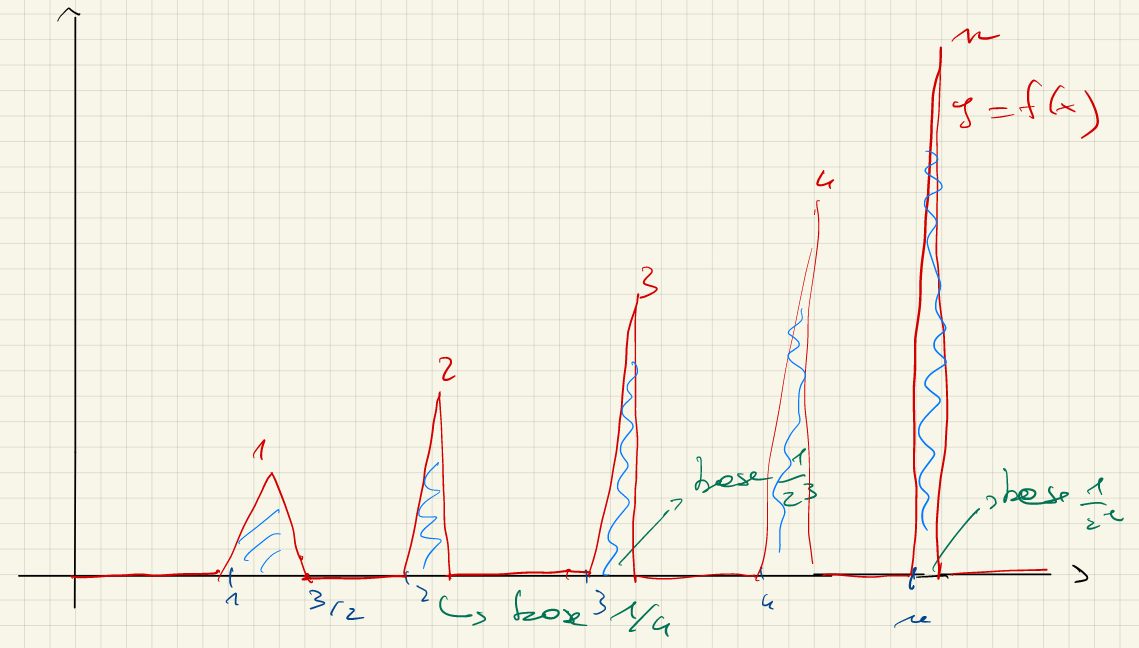
\includegraphics[width=\textwidth]{cosiappuntiti.png}
	\end{figure}
	
	Ad ogni numero naturale $n$ costruite un triangolo di base $\frac{1}{2^n}$ e altezza $n$
	
	\begin{empheq}{equation*}
		\int_{1}^{+\infty} f(x)dx = \sum (\text{aree dei triangoli}) = \sum_{n=1}^{\infty} \frac{1}{2} \frac{1}{2^n} \cdot n = \frac{1}{2} \sum_{n=1}^{\infty} \frac{n}{2^n}, 
	\end{empheq}
	che è una serie convergente.
	
	\paragraph{\textcolor{red}{Osservazione}}
	Se $f:[a,b] \rightarrow \R$ è Riemann integrabile, allora è integrabile anche in senso improprio e i due integrali coincidono.
	
	\paragraph{\textcolor{red}{Definizione}}
	$f:[a,b] \rightarrow \R,\,\, a,b \in \R \cup \{\pm \infty\}$, Riemann integrabile in $[c,d]\,\, \forall a<c<d<b$. $f$ si dice integrabile in senso improprio in $ ]a,b[$ se, fissato $\xi \in ]a,b[$, lo è in $]a, \xi]$ e in $[\xi,b[$ \textcolor{orange}{(esistono finiti $\lim_{c \rightarrow a^+} \int_{c}^{\xi} f(x)dx$ e $\lim_{d\rightarrow b^-}\int_{\xi}^{d} f(x)dx$)} e in tal caso si pone 
	\begin{empheq}{equation*}
		\int_{a}^{b} f(x)dx = \int_{a}^{\xi} f(x)dx + \int_{\xi}^{b} f(x) dx
	\end{empheq}
	Si verifica che la definizione non dipende da punto $\xi$ fissato.
	
	
	\paragraph{\textcolor{red}{Esempio}}
	Come si integra $\int_{-\infty}^{+\infty} \frac{1}{1+x^2}dx$?\\
	$x \mapsto \frac{1}{1+x^2}$ è integrabile secondo Riemann in $[c,d] \,\, \forall c<d$. \\
	Sia $\xi = 2$. Dobbiamo verificare se la funzione è integrabile in senso improprio in $]-\infty,2] $ e in $ [2, +\infty[$
	\begin{empheq}{align*}
		&\int_{-\infty}^{2}\frac{1}{1-x^2}dx = \lim_{c \rightarrow -\infty} \int_{c}^{2} \frac{1}{1+x^2}dx = \lim_{c \rightarrow -\infty} \left(\arctan{2+\frac{\pi}{2}}\right)= \arctan{2+\frac{\pi}{2}}\\
		&\int_{2}^{+\infty}\frac{1}{1-x^2} dx =\lim_{c \rightarrow +\infty} \int_{2}^{c} \frac{1}{1-x^2}dx=\lim_{c \rightarrow +\infty} (\arctan{c}-\arctan{2})=\frac{\pi}{2}-\arctan{2}\\
		&\Rightarrow \int_{-\infty}^{+\infty} \frac{1}{1+x^2}dx \,\,\,\, \text{converge e}\,\,\, \int_{-\infty}^{+\infty}\frac{1}{1+x^2}dx = \int_{-\infty}^{2}\frac{1}{1+x^2} dx+ \int_{2}^{+\infty}\frac{1}{1+x^2}dx
	\end{empheq}
	
	\paragraph{\textcolor{red}{Esempio}}
	\begin{empheq}{align*}
		&f(x)=\frac{1}{x^\alpha}, \,\,\,\,\,x \in ]0,+\infty[\\
		&\alpha > 0 \Rightarrow \lim_{x \rightarrow 0^+} f(x)=+\infty.
	\end{empheq}
	Preso $\xi=1$, $f$ è integrabile in senso improprio in $]0,+\infty[ \Leftrightarrow$ entrambi gli integrali $\int_{0}^{1} \frac{1}{x^\alpha} dx$ e $\int_{1}^{+\infty} \frac{1}{x^\alpha} dx$ convergono ma
	\begin{empheq}{align*}
		&\int_{0}^{1}\frac{1}{x^\alpha}dx \,\,\,\,\, \text{converge} \Leftrightarrow \alpha <1 \\
		& \int_{1}^{+\infty} \frac{1}{x^\alpha}dx \,\,\,\,\, \text{converge} \Leftrightarrow \alpha > 1\\
		& \Rightarrow \int_{0}^{+\infty} \frac{1}{x^\alpha}dx \,\,\,\text{non converge per alcun valore di} \,\, \alpha
	\end{empheq}
	
	\paragraph{\textcolor{red}{Esempio}}
	\begin{empheq}{equation*}
		f(x)= 
		\begin{cases}
			& e^x\,\,\,\,\, \text{se} x \leq 1 \\
			& \frac{1}{x \sqrt{x-1}}\,\,\,\,\, \text{se}\,\,\, x>1
		\end{cases}
	\end{empheq}
	vogliamo stabilire se $\int_{-\infty}^{+\infty}f(x)dx$ converge.\\
	\begin{figure}[h!]
		\centering
		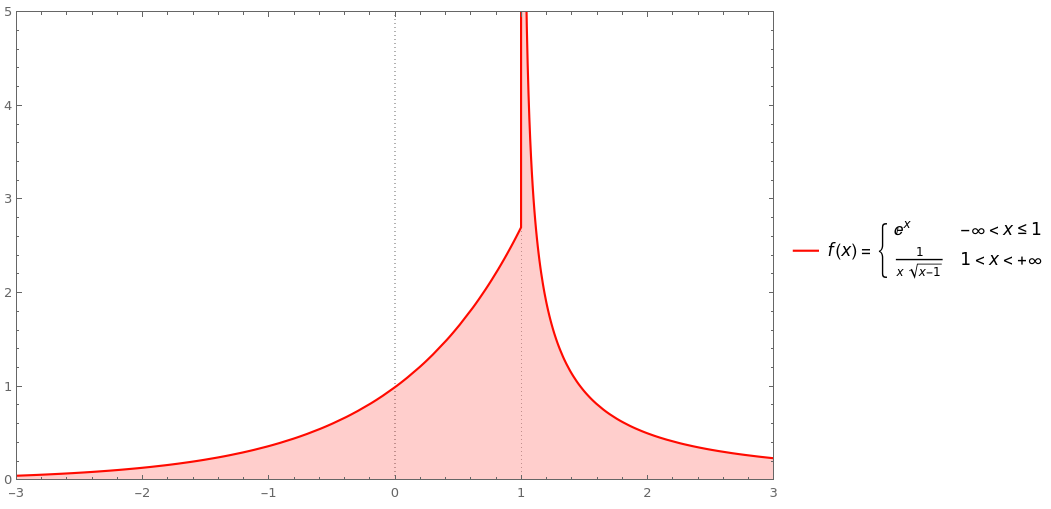
\includegraphics[width=\textwidth]{espefrac.png}
	\end{figure}
	
	Devo studiare $\int_{-\infty}^{1}f(x) dx = \int_{-\infty}^{1}e^x dx$ e, prendendo $\xi=3$,  $\int_{1}^{3}f(x)dx$ e $\int_{3}^{+\infty}f(x)dx$. Se tutti convergono, anche $\int_{-\infty}^{+\infty} f(x)dx$ converge e 
	\begin{empheq}{equation*}
		\int_{-\infty}^{+\infty} f(x)dx = \int_{-\infty}^{1} f(x)dx + \int_{1}^{3} f(x)dx + \int_{3}^{+\infty} f(x)dx
	\end{empheq}
	
	\paragraph{\textcolor{red}{Ulteriore Definizione}}
	In generale, data $f:]a,b[\rightarrow \R$ integrabile in senso improprio in $]x_0,x_1[,]x_1,x_2[,...,]x_{n-1},x_n[$ con $a= x_0 <x_1<...<x_n=b$, allora $f$ si dice integrabile in senso improprio in $]a,b[$ e si pone 
	\begin{empheq}{equation*}
		\int_{a}^{b}f(x)dx= \sum_{i=1}^{n} \int_{x_{i-1}}^{x_i}f(x)dx.
	\end{empheq}
	
	
	
\end{comment}